\section{Evaluation Plan} \label{sec:eval}

To evaluate our algorithms, we decided to use the ``scikit-learn''
\citep{scikit-learn} package for Python. In exploring the best way to
map workloads onto benchmarks, we evaluated both clustering algorithms
as well as SVM. The rest of this section discusses the results we
observed with each method.

Clustering was our first approach as an unsupervised algorithm seemed
to best fit the data at hand. As such, we tried the following methods,
all of which are inbuilt in scikit-learn:

\begin{itemize}
\item K-Mean
\item Affinity Propagation
\item Mean-Shift
\item Ward Agglomerative Clustering
\item DBSCAN
\end{itemize}

\begin{figure}[p]
    \centering
    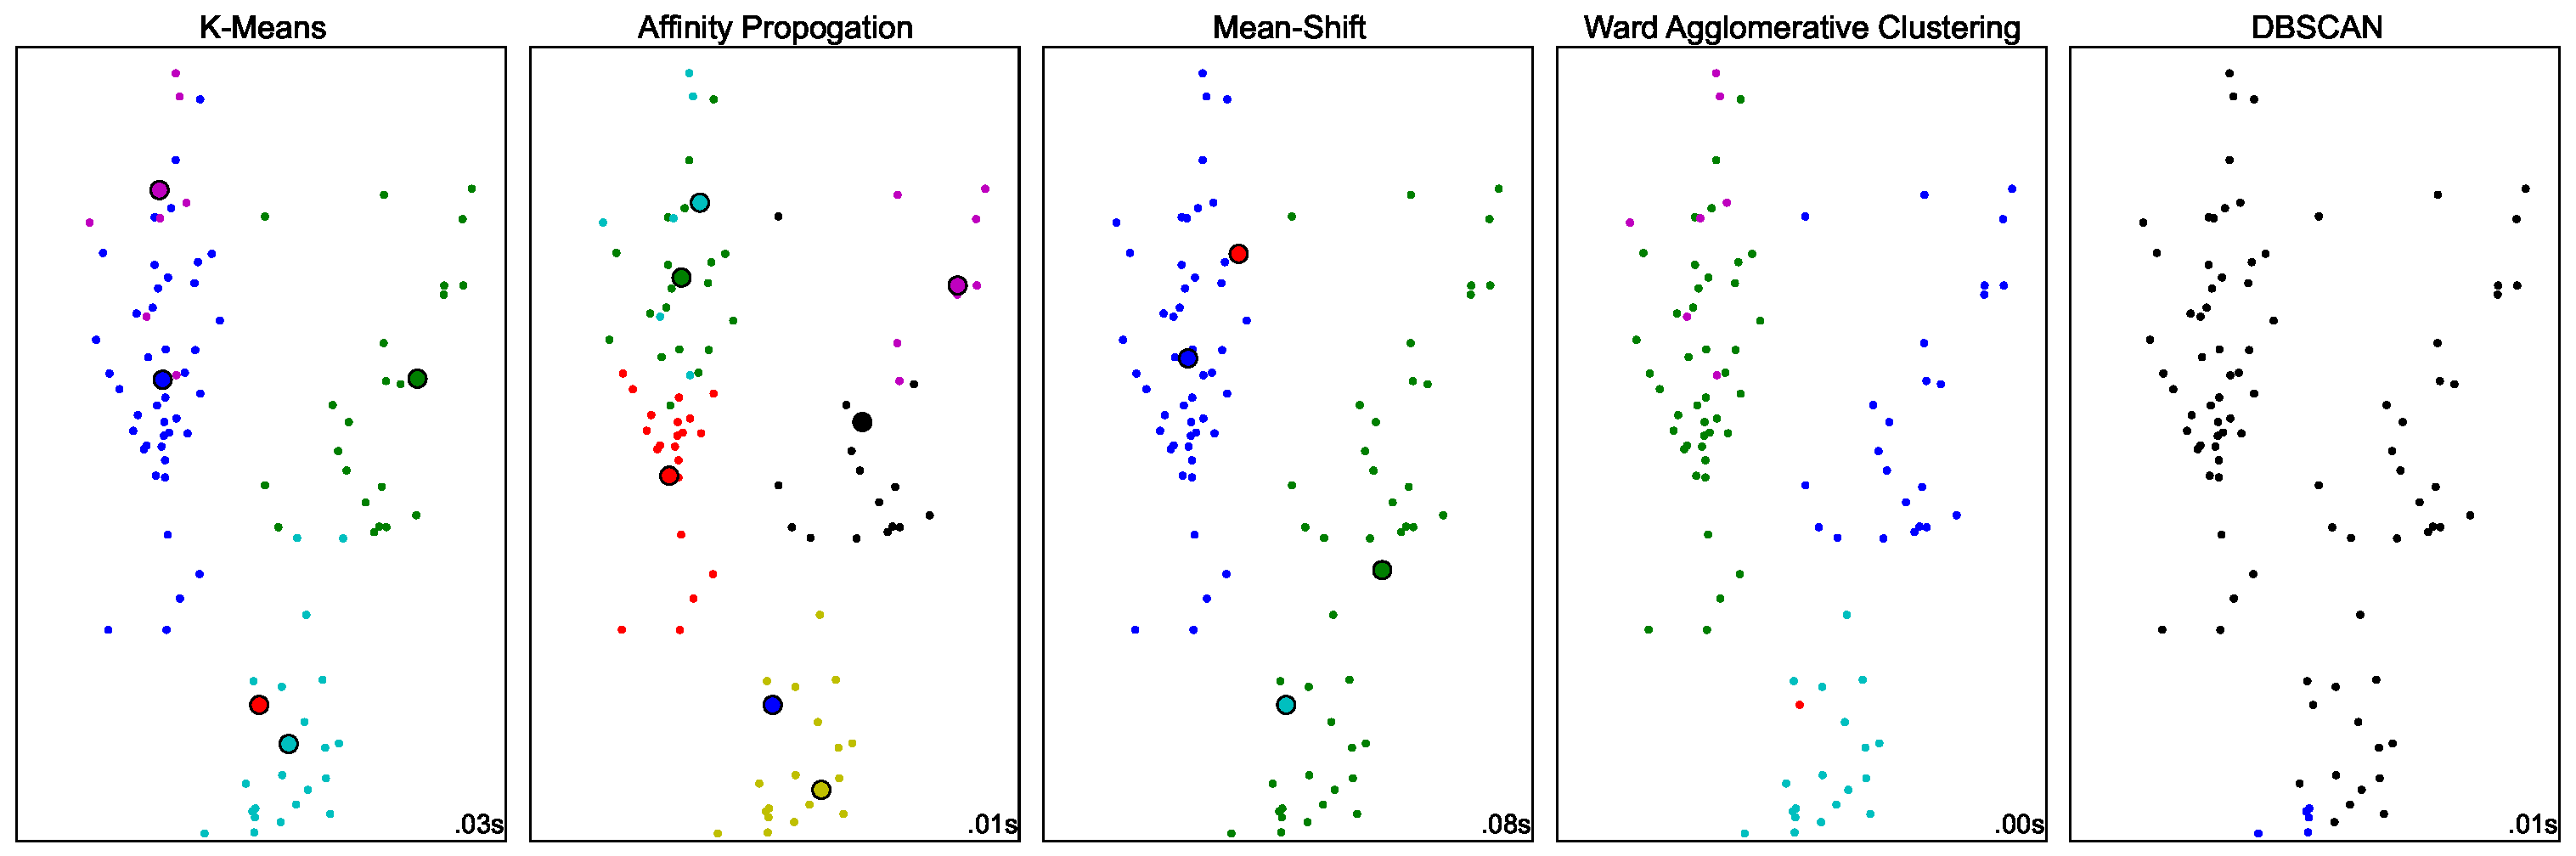
\includegraphics[width=0.8\textwidth]{clustering.eps}
    \caption{Clusters Found by the Clustering Algorithms}
    \label{fig:clusters}
\end{figure}

\begin{figure}[p]
    \centering
    \begin{tabular}{c c c c}
      \toprule
      Algorithm                     & Homogeneity & Completeness & V-Measure \\
      \midrule
      K-Means                       & 1.000       & 1.000        & 1.000     \\
      Affinity-Propagation          & 0.824       & 1.000        & 0.904     \\
      Mean-Shift                    & 1.000       & 0.795        & 0.886     \\
      Ward Agglomerative Clustering & 1.000       & 1.000        & 1.000     \\
      DBSCAN                        & 0.000       & 1.000        & 0.000     \\
      \bottomrule
    \end{tabular}

    \caption{Clustering Algorithm Performance Metrics}
    \label{fig:clustering-metrics}
\end{figure}

The clusters found by each algorithm can be seen in
\ref{fig:clusters}. We also calculated common clustering metrics such
as homogeneity, completeness, and V-measure. These results can be
found in \ref{fig:clustering-metrics}. From the results, we notice
immediately that DBSCAN does not work well with our data. Indeed, it
does not find any distinct clusters at all. However, K-Means and Ward
Agglomerative Clustering are very good. We believe that this is
partially because both of these algorithms require number of clusters
as a parameter, which allows them to find our desired number of
clusters. However, this is not a restriction for our problem as we
know the number of benchmarks - and hence the number of clusters -
that we have.

In addition to evaluating clustering algorithms, we also evaluated
Support Vector Machines, a supervised classifier. While real-world
data will not be labeled and hence a supervised classifier cannot be
used, it is useful to see how effective our features are in
discriminating between benchmarks. Using a simple two-fold
cross-validation, we found that a simple SVM with an RBF kernel
achieved 86\% precision but with a very high standard deviation of
28\%. However, this is still a very strong result as it indicates that
our features effectively separate our data into our desired
classes. While it is not clear that our features are still useful with
heterogeneous real-world workloads, we are hopeful that they are.
